\documentclass[aspectratio=169]{beamer}
\usetheme{simple}

\input{preamble/preamble.tex}
\input{preamble/preamble_math.tex}
% \input{preamble/preamble_acronyms.tex}

\title{Lecture 3: Exponential Family Distributions}
\subtitle{STATS305B: Applied  Statistics II}
\author{Scott Linderman}
\date{\today}


\begin{document}


\maketitle
    
\begin{frame}{Recap}

Last time...
\begin{itemize}
    \item Logistic Regression
    \item Maximum Likelihood Estimation via Gradient Descent, Newton's Method, and IRLS
    \item Regularization and Converge Rates
\end{itemize}

\end{frame}
    
\begin{frame}{Outline}

    Today...
    \begin{itemize}
        \item Definition and Examples
        \item The Log Normalizer
        \item Maximum Likelihood Estimation
        \item Mean Parameterization
        \item KL Divergence and Deviance Residuals
    \end{itemize}
    
\end{frame}
    
    
    
\begin{frame}[t,allowframebreaks]{Exponential Families}\label{exponential-families}
\begin{center}
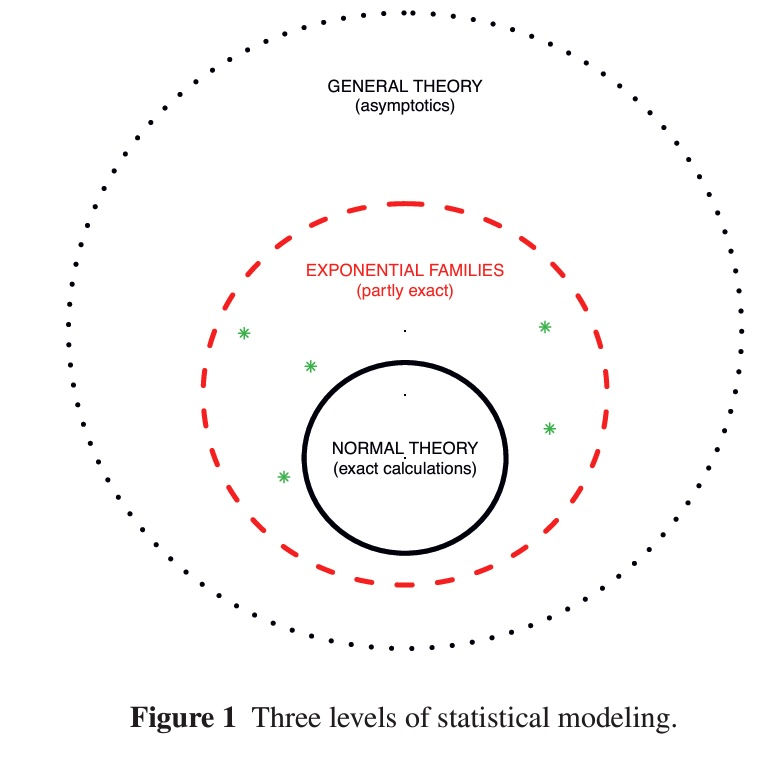
\includegraphics[width=.4\textwidth]{04_expfam/efron_levels.jpg}
\end{center}
From Efron (2022).
\end{frame}


\begin{frame}[t,allowframebreaks]{Definition}\label{definition}

Exponential family distributions have densities of the form,
\begin{align*}
    p(y; \eta) &= h(y) \exp \left \{\langle t(y), \eta \rangle - A(\eta) \right\},
\end{align*} where 
\begin{itemize}
    \item \(h(y): \cY \to \reals_+\) is the \textbf{base measure}, 
    \item \(t(y) \in \reals^T\) are the \textbf{sufficient statistics}, 
    \item \(\eta \in \reals^T\) are the \textbf{natural parameters}, and 
    \item \(A(\eta): \reals^T \to \reals\) is the \textbf{log normalizing} function (aka the \textbf{partition function}).
\end{itemize}

The log normalizer ensures that the density is properly normalized,
\begin{align*}
    A(\eta) &= \log \int h(y) \exp \left \{\langle t(y), \eta \rangle \right\} \dif y
\end{align*}

The domain of the exponential family is the set of valid natural
parameters, \(\Omega = \{\eta: A(\eta) < \infty\}\). An exponential
family is a family of distributions defined by base measure \(h\) and
sufficient statistics \(t\), and it is indexed by natural paremeters
\(\eta \in \Omega\).
\end{frame}


% \begin{frame}[t,allowframebreaks]{Example Gaussian with known
% variance}\label{gaussian-with-known-variance}

% Consider the scalar Gaussian distribution, \begin{align*}
% \mathrm{N}(y; \mu, \sigma^2) 
% &= \frac{1}{\sqrt{2 \pi \sigma^2}} e^{-\frac{1}{2\sigma^2} ( y- \mu)^2} \\
% &= \frac{1}{\sqrt{2 \pi \sigma^2}} e^{-\frac{1}{2\sigma^2} ( y^2 - 2 y \mu + \mu^2)}
% \end{align*} We can write this as an exponential family distribution
% where, where 
% \begin{itemize}
%     \item the base measure is
% \(h(y) = \frac{e^{-\frac{y^2}{2 \sigma^2}}}{\sqrt{2 \pi \sigma^2}}\) 
%     \item the sufficient statistics are \(t(y) = \frac{y}{\sigma}\) 
%     \item the natural parameter is \(\eta = \frac{\mu}{\sigma}\) 
%     \item  the log normalizer is \(A(\eta) = \frac{\eta^2}{2}\) 
%     \item the domain is \(\Omega = \reals\)
% \end{itemize}
% \end{frame}

\begin{frame}[t,allowframebreaks]{Example: Poisson distribution}\label{poisson-distribution}

Take the Poisson pmf, \begin{align*}
    \mathrm{Po}(y; \lambda) 
    &= \frac{1}{y!} \lambda^{y} e^{-\lambda} \\
    &= \frac{1}{y!} \exp \left\{ y \log \lambda - \lambda \right \} \\
    &= h(y) \exp \left\{ y \eta - A(\eta) \right \} 
\end{align*} 
where 
\begin{itemize}
    \item the base measure is \(h(y) = \frac{1}{y!}\) 
    \item the sufficient statistics are \(t(y) = y\) 
    \item the natural parameter is \(\eta = \log \lambda\) 
    \item the log normalizer is \(A(\eta) = \lambda = e^\eta\) % and the domain is \(\Omega = \reals\)
\end{itemize}
\end{frame}

\begin{frame}[t,allowframebreaks]{Bernoulli distribution}\label{bernoulli-distribution}

\textbf{Exercise:} Write the Bernoulli distribution in
exponential family form. Recall that its pmf is \begin{align*}
    \mathrm{Bern}(y; p) &= p^{y} \, (1-p)^{1 - y} 
\end{align*} What are the base measure, the sufficient statistics, the
natural parameter, the log normalizer, and the domain? 

Submit your answers here,
\begin{center}
    \textbf{\textcolor{blue}{\url{https://tinyurl.com/stats305blec03}}}
\end{center}
\end{frame}

\begin{frame}[t,allowframebreaks]{Categorical distribution}\label{categorical-distribution}

Finally, take the categorical pmf for \(Y \in \{1, \ldots, K\}\),
\begin{align*}
    \mathrm{Cat}(y; \mbpi) 
    &= \prod_{k=1}^K \pi_k^{\bbI[y = k]} \\
    &= \exp \left\{ \sum_{k=1}^K \bbI[y=k], \log \pi_k \right \} \\
    &= \exp \left\{ \langle \mbe_y, \log \mbpi \rangle \right \} \\
    &= h(y) \exp \left\{ \langle t(y), \mbeta \rangle - A(\mbeta) \right \} 
\end{align*} where 
\begin{itemize}
    \item the base measure is \(h(y) = \bbI[y \in \{1,\ldots,K\}]\) 
    \item the sufficient statistics are \(t(y) = \mbe_y\), the one-hot vector representation of \(y\) 
    \item the natural parameter is \(\mbeta = \log \mbpi = (\log \pi_1, \ldots, \log \pi_K)^\top \in \reals^K\)
    \item the log normalizer \(A(\mbeta) = 0\) 
    \item the domain is \(\Omega = \reals^K\)
\end{itemize}
\end{frame}

\begin{frame}[t,allowframebreaks]{The Log Normalizer}\label{the-log-normalizer}

The \textbf{cumulant generating function} --- i.e., the log of the
moment generative function --- is a difference of log normalizers,
\begin{align*}
\log \E_\eta[e^{\langle t(Y), \theta \rangle}] 
&= \log \int h(y) \exp \left\{ \langle t(y), \eta + \theta \rangle - A(\eta) \right\} \dif y \\
&= \log e^{A(\eta + \theta) - A(\eta)} \\
&= A(\eta + \theta) - A(\eta) \\
&\triangleq K_\eta(\theta)
\end{align*} Its derivatives (with respect to \(\theta\) and evaluated
at zero) yield the cumulants. In particular, 
\begin{itemize}
    \item \(\nabla_\theta K_\eta(0) = \nabla A(\eta)\) yields the first cumulant
of \(t(Y)\), its mean 
    \item \(\nabla^2_\theta K_\eta(0) = \nabla^2 A(\eta)\) yields the second cumulant, its covariance
\end{itemize}

Higher order cumulants can be used to compute skewness, kurtosis, etc.
\end{frame}

\begin{frame}[t,allowframebreaks]{Gradient of the log
normalizer}\label{gradient-of-the-log-normalizer}

We can also obtain this result more directly. \begin{align*}
    \nabla A(\eta) 
    &= \nabla \log \int h(y) \exp \left \{\langle t(y), \eta \rangle \right\} \dif y \\
    &= \frac{\int h(y) \exp \left \{\langle t(y), \eta \rangle \right\} t(y) \dif y}{\int h(y) \exp \left \{\langle t(y), \eta \rangle \right\} \dif y} \\
    &= \int p(y \mid \eta) \, t(y) \dif y \\
    &= \E_\eta[t(Y)]
\end{align*} Again, the gradient of the log normalizer yields the
\textbf{expected sufficient statistics},
\end{frame}

\begin{frame}[t,allowframebreaks]{Hessian of the log
normalizer}\label{hessian-of-the-log-normalizer}

The Hessian of the log normalizer yields the \textbf{covariance of the
sufficient statistics}, \begin{align*}
    \nabla^2 A(\eta) 
    &= \nabla \int p(y \mid \eta) \, t(y) \dif y \\
    &= \int p(y \mid \eta) \, t(y) \, (t(y) - \nabla A(\eta))^\top \dif y \\
    &= \E[t(Y) t(Y)^\top ] - \E[t(Y)] \, \E[t(Y)]^\top \\
    &= \mathrm{Cov}[t(Y)]
\end{align*}
\end{frame}

\begin{frame}[t,allowframebreaks]{Maximum Likelihood
Estimation}\label{maximum-likelihood-estimation}

Suppose we have \(y_i \iid\sim p(y; \eta)\) for a minimal exponential
family distribution with natural parameter \(\eta\). The log likelihood
is, \begin{align*}
\cL(\eta)
&= \sum_{i=1}^n \log p(y_i; \eta) \\
&= \left \langle \sum_{i=1}^n t(y_i), \eta \right \rangle - n A(\eta) + c
\end{align*} The gradient is \begin{align*}
\nabla \cL(\eta)
&= \sum_{i=1}^n t(y_i) - n \nabla A(\eta),
\end{align*} and the Hessian is
\(\nabla^2 \cL(\eta) = -n \nabla^2 A(\eta)\).

Since the log normalizer is convex, all local optima are global. If the
log normalizer is \emph{strictly} convex, the MLE will be unique.

Setting the gradient to zero and solving yields the stationary
conditions for the MLE, \begin{align*}
\nabla A[\hat{\eta}_{\mathsf{MLE}}] &= \bbE[t(Y); \hat{\eta}_{\mathsf{MLE}}] 
= \frac{1}{n} \sum_{i=1}^n t(y_i).
\end{align*} When \(\nabla A\) is invertible, the MLE is unique,
\begin{align*}
\hat{\eta}_{\mathsf{MLE}} = [\nabla A]^{-1} \left( \frac{1}{n} \sum_{i=1}^n t(y_i) \right).
\end{align*} 

Even if \(\nabla A\) is not invertible, maximum likelihood
estimation amounts to matching empirical means of the sufficient
statistics to corresponding natural parameters.
\end{frame}

\begin{frame}[t,allowframebreaks]{Asymptotic normality}\label{asymptotic-normality}

Recall that the MLE is asymptotically normal with variance given by the
inverse Fisher information.

For an exponential family distribution, the Fisher information is,
\begin{align*}
\cI(\eta) &= - \E[\nabla^2 \log p(y_i; \eta)] = \nabla^2 A(\eta) = \Cov_\eta[t(Y)].
\end{align*} 
Thus, 
\begin{align*}
    \sqrt{n} (\hat{\eta}_{\mathsf{MLE}} - \eta) \to \mathrm{N}(0, \cI(\eta)^{-1}) 
    = \mathrm{N}(0, \Cov_\eta[t(Y)]^{-1})
\end{align*}
\end{frame}

\begin{frame}[t,allowframebreaks]{Example: MLE for the Poisson
distribution}\label{example-mle-for-the-poisson-distribution}

Suppose \(Y_i \iid{\sim} \mathrm{Po}(\lambda)\) for \(i=1,\ldots,n\).
The natural parameter of the Poisson distribution is
\(\eta = \log \lambda\), and the maximum likelihood estimate is
\(\hat{\eta}_{\mathsf{MLE}} = \log \left(\frac{1}{n} \sum_{i=1}^n y_i \right)\).
The Fisher information matrix is the variance,
\(\cI(\eta) = \mathrm{Var}_\eta[Y] = e^\eta\).

\begin{center}
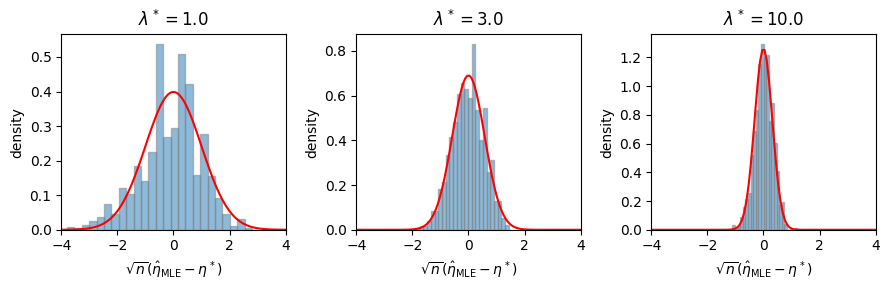
\includegraphics[width=.9\textwidth]{04_expfam/output_14_0.png}
\end{center}
\end{frame}

\begin{frame}[t,allowframebreaks]{Minimal Exponential
Families}\label{minimal-exponential-families}

The Hessian of the log normalizer gives the covariance of the sufficient
statistic. Since covariance matrices are positive semi-definite, the
\emph{log normalizer is a convex function} on \(\Omega\).

If the covariance is strictly positidive definite --- i.e., if the
minimum eigenvalue of \(\nabla^2 A(\eta)\) is strictly greater than zero
for all \(\eta \in \Omega\) --- then the log normalizer is
\emph{strictly} convex. In that case, we say that the exponential family
is \textbf{minimal}

\textbf{Question:} Is the exponential family representation of
the categorical distribution above a minimal representation? If not, how
could you encode it in minimal form?

\end{frame}

\begin{frame}[t,allowframebreaks]{Mean Parameterization}\label{mean-parameterization}

When constructing models with exponential family distributions, like the
generalized linear models below, it is often more convenient to work
with the \textbf{mean parameters} instead. for a \(d\)-dimensional
sufficient statistic, let, \begin{align*}
\cM &\triangleq \left\{ \mu \in \reals^d : \exists \, p \text{ s.t. } \E_p[t(Y)] = \mu \right\}
\end{align*} denote the set of mean parameters realizable \emph{by any
distribution} \(p\).

Two facts: 
\begin{enumerate}
    \item The gradient mapping \(\nabla A: \Omega \mapsto \cM\) is
\emph{injective} (one-to-one) if and only if the exponential family is
minimal. 
    \item The gradient is a \emph{surjective} mapping from mean
parameters to the \emph{interior} of \(\cM\). All mean parameters in the
interior of \(\cM\) (excluding the boundary) can be realized by an
exponential family distribution. (Mean parameters on the boundary of
\(\cM\) can be realized by a limiting sequence of exponential family
distributions.)
\end{enumerate}

Together, these facts imply that the gradient of the log normalizer
defines a \emph{bijective} map from \(\Omega\) to the interior of
\(\cM\) for minimal exponential families.

For minimal families, we can work with the mean parameterization
instead, 
\begin{align*}
p(y; \mu) 
&= h(y) \exp \left\{ \langle t(y), [\nabla A]^{-1}(\mu) \rangle - A([\nabla A]^{-1}(\mu)) \right\}.
\end{align*} 
for mean parameters \(\mu\) in the interior of \(\cM\).
\end{frame}

\begin{frame}[t,allowframebreaks]{MLE for the Mean
Parameters}\label{mle-for-the-mean-parameters}

Alternatively, consider the maximum likelihood estimate of the mean
parameter \(\mu \in \cM\). Before doing any math, we might expect the
MLE to be the empirical mean. Indeed, that is the case. To simplify
notation, let \(\eta(\mu) = [\nabla A]^{-1}(\mu)\). The log likelihood,
\begin{align*}
\cL(\mu)
&= \left \langle \sum_{i=1}^n t(y_i), \eta(\mu) \right \rangle - n A(\eta(\mu)) + c
\end{align*} has gradient, \begin{align*}
\nabla \cL(\mu)
&= \left(\frac{\partial \eta}{\partial \mu}(\mu) \right) \left[\sum_{i=1}^n t(y_i) - n \nabla A(\eta(\mu))\right] \\
&= \left(\frac{\partial \eta}{\partial \mu}(\mu) \right) \left[\sum_{i=1}^n t(y_i) - n \mu \right],
\end{align*} where \(\tfrac{\partial \eta}{\partial \mu}(\mu)\) is the
Jacobian of inverse gradient mapping at \(\mu\). Assuming the Jacobian
is positive definite, we immediately see that, \begin{align*}
\hat{\mu}_{\mathsf{MLE}} &= \frac{1}{n} \sum_{i=1}^n t(y_i).
\end{align*}

Now back to the Jacobian\ldots{} applying the
\href{https://en.wikipedia.org/wiki/Inverse_function_theorem}{inverse
function theorem}, shows that it equals the inverse covariance matrix,
\begin{align*}
\frac{\partial \eta}{\partial \mu} (\mu) 
= \frac{\partial [\nabla A]^{-1}}{\partial \mu} (\mu)
= [\nabla^2 A ([\nabla A]^{-1}(\mu))]^{-1} 
= \Cov_{\eta(\mu)}[t(Y)]^{-1},
\end{align*} which is indeed positive definite for minimal exponential
families.
\end{frame}

\begin{frame}[t,allowframebreaks]{Asymptotic normality}\label{asymptotic-normality}

We obtain the Fisher information of the mean parameter \(\mu\) by left
and right multiplying by the Jacobian, \begin{align*}
\cI(\mu) 
&= \left( \frac{\partial \eta}{\partial \mu} (\mu) \right)^\top \cI(\eta(\mu)) \left( \frac{\partial \eta}{\partial \mu} (\mu) \right) \\
&= \Cov_{\eta(\mu)}[t(Y)]^{-1} \Cov_{\eta(\mu)}[t(Y)] \Cov_{\eta(\mu)}[t(Y)]^{-1} \\
&= \Cov_{\eta(\mu)}[t(Y)]^{-1}.
\end{align*}

Thus, the MLE of the mean parameter is asymptotically normal with
covariance determined by the inverse Fisher information,
\(\cI(\mu)^{-1} = \Cov_{\eta(\mu)}[t(Y)]\). More formally,
\begin{align*}
\sqrt{n} \left( \hat{\mu}_{\mathsf{MLE}} - \mu^\star \right) 
&\to \mathrm{N}(0, \Cov_{\eta(\mu)}[t(Y)])
\end{align*} As usual, to derive confidence intervals we plug in the MLE
to evaluate the asymptotic covariance.

Compare this result to the asymptotic covariances we computed in Lecture
1 for the Bernoulli distribution. Recall that for
\(X_i \iid\sim \mathrm{Bern}(\theta)\), where \(\theta \in [0,1]\) is
the mean parameter, we found, \begin{align*}
\sqrt{n} (\hat{\theta}_{\mathsf{MLE}} - \theta^\star) \to \mathrm{N}\left(0, \Var_\theta[X] \right).
\end{align*} Now we see that this is a general property of exponential
family distributions.
\end{frame}

\begin{frame}[t,allowframebreaks]{Revisiting the Poisson
example}\label{revisiting-the-poisson-example}

Revisiting the example above, here we have
\(\hat{\lambda}_{\mathsf{MLE}} = \frac{1}{n} \sum_i y_i\) and
\(\cI(\lambda) = \mathrm{Var}_\lambda[Y]^{-1} = \frac{1}{\lambda}\). We
expect, \begin{align*}
\sqrt{n}(\hat{\lambda}_{\mathsf{MLE}} - \lambda) \rightarrow \mathrm{N}(0, \cI(\lambda)^{-1}) = \mathrm{N}(0, \lambda).
\end{align*}

\begin{center}
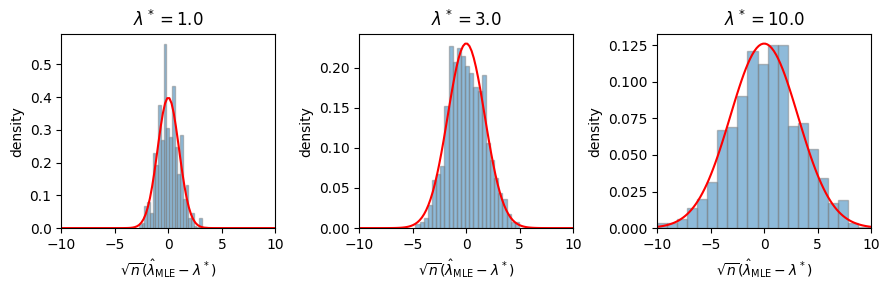
\includegraphics[width=.9\textwidth]{04_expfam/output_20_0.png}
\end{center}

\end{frame}

\begin{frame}[t,allowframebreaks]{Conjugate duality}\label{conjugate-duality}

The log normalizer is a convex function. Its conjugate dual is,
\begin{align*}
A^*(\mu) &= \sup_{\eta \in \Omega} \left\{ \langle \mu, \eta \rangle - A(\eta) \right\}
\end{align*} We recognize this as the maximum likelihood problem mapping
expected sufficient statistics \(\mu\) to natural parameters \(\eta\).
For minimal exponential families, the supremum is uniquely obtained at
\(\eta(\mu) = [\nabla A]^{-1}(\mu)\). The conjugate dual evaluates to
the log likelihood obtained at \(\eta(\mu)\).

It turns out the conjugate dual is also related to the entropy; in
particular, for any \(\mu\) in the interior of \(\cM\), \begin{align*}
A^*(\mu) = - \bbH[p_{\eta(\mu)}],
\end{align*} where \(\eta(\mu) = [\nabla A]^{-1}(\mu)\) for minimal
exponential families. To see this, note that \begin{align*}
-\bbH[p_{\eta(\mu)}] 
&= \bbE_{p(\eta(\mu))}[\log p(X; \eta(\mu))] \\
&= \bbE_{p(\eta(\mu))}[\langle t(X), \eta(\mu) \rangle - A(\eta(\mu))] \\
&= \langle \mu, \eta(\mu) \rangle - A(\eta(\mu)) \\
&= A^*(\mu).
\end{align*}

Moreover, for minimal exponential families, the gradient of \(A^*\)
provides the inverse map from mean parameters to natural parameters,
\begin{align*}
\nabla A^*(\mu) &= \arg \max_{\eta \in \Omega} \left\{ \langle \mu, \eta \rangle - A(\eta) \right\} 
= [\nabla A]^{-1}(\mu).
\end{align*}

Finally, the log normalizer has a variataional representation in terms
of its conjugate dual, \begin{align*}
A(\eta) &= \sup_{\mu \in \cM} \left\{ \langle \mu, \eta \rangle - A^*(\mu) \right\}.
\end{align*}

For more on conjugate duality, see
Wainwright and Jordan (2008), ch.~3.6.
\end{frame}

\begin{frame}[t,allowframebreaks]{KL Divergence}\label{kl-divergence}

The \textbf{Kullback-Leibler (KL) divergence}, or \textbf{relative
entropy}, between two distributions is, \begin{align*}
\KL{p}{q} &= \E_{p}\left[\log \frac{p(Y)}{q(Y)} \right].
\end{align*} It is non-negative and equal to zero if and only if
\(p = q\). The KL divergence is \emph{not} a distance because it is not
a symmetric function of \(p\) and \(q\). (generally,
\(\KL{p}{q} \neq \KL{q}{p}\).)

When \(p\) and \(q\) belong to the same exponential family with natural
parameters \(\eta_p\) and \(\eta_q\), respectively, the KL simplifies
to, \begin{align*}
\KL{p}{q} 
&= \E_{p}\left[ \langle t(Y), \eta_p \rangle - A(\eta_p) - \langle t(Y), \eta_q \rangle + A(\eta_q) \right] \\
&= \langle \E_{p} [t(Y)], \eta_p - \eta_q \rangle - A(\eta_p) + A(\eta_q) \\
&= \langle \nabla A(\eta_p), \eta_p - \eta_q \rangle - A(\eta_p) + A(\eta_q).
\end{align*} This form highlights that the KL divergence between
exponential family distributions is a special case of a
\href{https://en.wikipedia.org/wiki/Bregman_divergence}{\textbf{Bregman
divergence}} based on the convex function \(A\).
\end{frame}

\begin{frame}[t,allowframebreaks]{Example: Poisson Distribution}

Consider the Poisson distribution with known mean \(\lambda\). In the
example above, we cast it as an exponential family distribution with -
sufficient statistics \(t(y) = y\) - natural parameter
\(\eta = \log \lambda\) - log normalizer \(A(\eta) = e^\eta\)

The KL divergence is,
\begin{align*}
\KL{p}{q} 
&= \langle e^{\eta_p}, \eta_p - \eta_q \rangle - e^{\eta_p} + e^{\eta_q} \\
&= \lambda_p \log \frac{\lambda_p}{\lambda_q} - \lambda_p + \lambda_q \\
\end{align*} 
\end{frame}


% \begin{frame}[t,allowframebreaks]{Example: Gaussian Distribution}

% Consider the scalar Gaussian distribution with known variance
% \(\sigma^2\). In the example above, we cast it as an exponential family
% distribution with - sufficient statistics \(t(y) = \frac{y}{\sigma}\) -
% natural parameter \(\eta = \frac{\mu}{\sigma}\) - log normalizer
% \(A(\eta) = \frac{\eta^2}{2}\)

% Derive the KL divergence between two Gaussians with equal variance.
% Denote their natural parameters by \(\eta_p = \frac{\mu_p}{\sigma}\) and
% \(\eta_q = \frac{\mu_q}{\sigma}\), respectively.

% :::\{admonition\} Answer :class: tip, dropdown The KL divergence is,
% \begin{align*}
% \KL{p}{q} 
% &= \langle \eta_p, \eta_p - \eta_q \rangle - \frac{\eta_p^2}{2} + \frac{\eta_q^2}{2} \\
% &=  \frac{\eta_p^2}{2} - \eta_p\eta_q + \frac{\eta_q^2}{2} \\
% &=  \frac{1}{2} (\eta_p - \eta_q)^2 \\
% &=  \frac{1}{2 \sigma^2} (\mu_p - \mu_q)^2.
% \end{align*} Note that here, the KL \emph{is} a symmetric function. 
% \end{frame}
    

\begin{frame}[t,allowframebreaks]{Deviance}\label{deviance}

Rearranging terms, we can view the KL divergence as a remainder in a
Taylor approximation of the log normalizer, \begin{align*}
A(\eta_q) 
&= A(\eta_p) + (\eta_q - \eta_p)^\top \nabla A(\eta_p) + \KL{p}{q}.
\end{align*} From this perspective, we see that the KL divergence is
related to the Fisher information, \begin{align*}
\KL{p}{q} 
&\approx \frac{1}{2} (\eta_q - \eta_p)^\top \nabla^2 A(\eta_p) (\eta_q - \eta_p) \\
&= \frac{1}{2} (\eta_q - \eta_p)^\top \cI(\eta_p) (\eta_q - \eta_p),
\end{align*} up to terms of order \(\cO(\|\eta_p - \eta_q\|^3)\).

Thus, while the KL divergence is not a distance metric due to its
asymmetry, it is approximately a squared distance under the Fisher
information metric, \begin{align*}
2 \KL{p}{q} \approx \|\eta_q - \eta_p\|_{\cI(\eta_p)}^2.
\end{align*} We call this quantity the \textbf{deviance}. It is simply
twice the KL divergence.
\end{frame}


\begin{frame}[t,allowframebreaks]{Deviance Residuals}

In a normal model, the standarized residual is
\(\frac{\hat{\mu} - \mu}{\sigma}\). We can view this as a function of
the deviance between two normals, \begin{align*}
\frac{\hat{\mu} - \mu}{\sigma} 
&= \mathrm{sign}(\hat{\mu} - \mu) \sqrt{2 \KL{\hat{\mu}}{\mu}}
\end{align*} where we have used the shorthand notation \begin{align*}
\KL{\mu}{\hat{\mu}} \triangleq \KL{\mathrm{N}(\mu, \sigma^2)}{\mathrm{N}(\hat{\mu}, \sigma^2)}.
\end{align*}

The same form generalizes to other exponential families as well, with
the \textbf{deviance residual} between the true and estimated mean
parameters defined as, \begin{align*}
r_{\mathsf{D}}(\hat{\mu}, \mu) &= \mathrm{sign}(\hat{\mu} - \mu) \sqrt{2 \KL{\hat{\mu}}{\mu}}.
\end{align*} One can show that deviance residuals tend to be closer to
normal than the more obvious Pearson residuals, \begin{align*}
r_{\mathsf{P}}(\hat{\mu}, \mu) &= \frac{\hat{\mu} - \mu}{\sqrt{\Var[t(Y); \hat{\mu}]}}.
\end{align*} For more on deviance residuals, see
 Efron (2022), ch.~1.
\end{frame}

\begin{frame}[t,allowframebreaks]{Revisiting the Poisson
example}\label{revisiting-the-poisson-example}

Finally, let's revisit the Poisson example one again. We already
computed the KL divergence between two Poisson distributions above,
\begin{align*}
\KL{\mathrm{Po}(\hat{\lambda})}{\mathrm{Po}(\lambda)}
&= \hat{\lambda} \log \frac{\hat{\lambda}}{\lambda} - \hat{\lambda} + \lambda,
\end{align*} so the deviance residual is, \begin{align*}
r_{\mathrm{D}}(\hat{\lambda}, \lambda) &= \mathrm{sign}(\hat{\lambda} - \lambda) \sqrt{2 \left(\hat{\lambda} \log \frac{\hat{\lambda}}{\lambda} - \hat{\lambda} + \lambda\right)}.
\end{align*} Compare this to the Pearon residual, \begin{align*}
r_{\mathrm{P}}(\hat{\lambda}, \lambda) &= \frac{\hat{\lambda} - \lambda}{\sqrt{\hat{\lambda}}}
\end{align*} Let's compare these residuals in simulation.

\begin{center}

\includegraphics[width=0.75\textwidth]{04_expfam/output_29_0.png}
\end{center}
\end{frame}
    
\begin{frame}[t,allowframebreaks]{Conclusion}\label{conclusion}

Exponential family distributions have many beautiful properties, and we've only scratched the surface. 

\begin{itemize}
    \item We'll see other nice properties when we talk about building probabilistic models for joint distributions of random variables using exponential family distributions, and conjugate relationships between exponential families will simplify many aspects of Bayesian inference. 
    \item We'll also see that inference in exponential families is closely connected to convex optimization --- we saw that today for the MLE! --- but for more complex models, the optimization problems can still be computationally intractable, even though its convex. That will motivate our discussion of variational inference later in the course.
\end{itemize}

Armed with exponential family distributions, we can start to build more expressive models for categorical data. First up, generalized linear models!
\end{frame}

    % Add a bibliography block to the postdoc
    
    
    
\end{document}
